\section{Complete display tables and season curves}
\label{app:displays}
Tables~\ref{tab:datasets}--\ref{tab:budgets} retain the exact counts, target identities, source conventions and denominator mappings behind the main figures. Figure~\ref{fig:nba} shows every NBA season. All displays are generated by \texttt{presentation/render.py}; the input and output manifest is in \texttt{presentation/README.md}.

\begin{table}[htbp]
\caption{\TabDatasetsCaption}
\label{tab:datasets}
\centering
\fontsize{8}{9}\selectfont
\begin{tabular}{llrrrr}
\toprule
Ranking & Original leader $>$ runner & $N$ & Ties (\%) & Min support & Clusters \\
\midrule
Arena & GPT-4-1106 $>$ GPT-4-0125 & 57,477 & 30.9 & 100 & 57,477 \\
MT human & GPT-4 $>$ Claude-v1 & 3,355 & 23.2 & 996 & 80 \\
MT GPT-4 & GPT-4 $>$ Claude-v1 & 2,400 & 25.0 & 800 & 80 \\
NBA 2006 & SAS $>$ DET & 1,230 & 0.0 & 82 & 164 \\
NBA 2007 & DAL $>$ PHO & 1,230 & 0.0 & 82 & 163 \\
NBA 2008 & BOS $>$ LAL & 1,230 & 0.0 & 82 & 162 \\
NBA 2009 & CLE $>$ LAL & 1,230 & 0.0 & 82 & 163 \\
NBA 2010 & CLE $>$ ORL & 1,230 & 0.0 & 82 & 164 \\
NBA 2011 & SAS $>$ CHI & 1,230 & 0.0 & 82 & 164 \\
NBA 2012 & SAS $>$ CHI & 990 & 0.0 & 66 & 120 \\
NBA 2013 & MIA $>$ OKC & 1,229 & 0.0 & 81 & 163 \\
NBA 2014 & SAS $>$ OKC & 1,230 & 0.0 & 82 & 163 \\
NBA 2015 & GSW $>$ ATL & 1,230 & 0.0 & 82 & 162 \\
\bottomrule
\end{tabular}

\end{table}

\begin{table}[htbp]
\caption{\TabPrimaryCaption}
\label{tab:primary}
\centering
\fontsize{8}{9}\selectfont
\begin{tabular}{lrrrrrr}
\toprule
Ranking & $N$ & $M$ & Decisive & Found $k$ & $100k/N$ (\%) & Gap [95\% range] \\
\midrule
Arena & 57,477 & 64 & 39,716 & 2 & 0.0035 & 0.008 [-0.094, 0.104] \\
MT human & 3,355 & 6 & 2,575 & 46 & 1.3711 & 0.376 [0.110, 0.642] \\
MT GPT-4 & 2,400 & 6 & 1,800 & 61 & 2.5417 & 0.809 [0.550, 1.113] \\
NBA 2006 & 1,230 & 30 & 1,230 & 1 & 0.0813 & 0.007 [-0.679, 0.694] \\
NBA 2007 & 1,230 & 30 & 1,230 & 5 & 0.4065 & 0.384 [-0.241, 1.038] \\
NBA 2008 & 1,230 & 30 & 1,230 & 5 & 0.4065 & 0.419 [-0.266, 1.109] \\
NBA 2009 & 1,230 & 30 & 1,230 & 2 & 0.1626 & 0.076 [-0.680, 0.957] \\
NBA 2010 & 1,230 & 30 & 1,230 & 2 & 0.1626 & 0.117 [-0.550, 0.746] \\
NBA 2011 & 1,230 & 30 & 1,230 & 1 & 0.0813 & 0.062 [-0.592, 0.753] \\
NBA 2012 & 990 & 30 & 990 & 2 & 0.2020 & 0.106 [-0.609, 0.976] \\
NBA 2013 & 1,229 & 30 & 1,229 & 3 & 0.2441 & 0.279 [-0.363, 0.924] \\
NBA 2014 & 1,230 & 30 & 1,230 & 4 & 0.3252 & 0.185 [-0.453, 0.820] \\
NBA 2015 & 1,230 & 30 & 1,230 & 8 & 0.6504 & 0.546 [-0.164, 1.322] \\
\bottomrule
\end{tabular}

\end{table}

\begin{table}[htbp]
\caption{\TabOnePercentCaption}
\label{tab:one_percent}
\centering
\fontsize{8}{9}\selectfont
\begin{tabular}{lrrrrrr}
\toprule
Ranking & $k$ & Random (\%) & Endpoint (\%) & Influence (\%) & Winner (\%) & Kendall (\%) \\
\midrule
Arena & 574 & 25.0 & 100.0 & 100.0 & 100.0 & 3.92 \\
MT human & 33 & 0.0 & 0.0 & 0.0 & 0.0 & 0.00 \\
MT GPT-4 & 24 & 0.0 & 0.0 & 0.0 & 0.0 & 0.00 \\
NBA 2006 & 12 & 38.2 & 100.0 & 100.0 & 100.0 & 2.99 \\
NBA 2007 & 12 & 0.0 & 100.0 & 100.0 & 100.0 & 2.53 \\
NBA 2008 & 12 & 0.0 & 100.0 & 100.0 & 100.0 & 3.22 \\
NBA 2009 & 12 & 13.0 & 100.0 & 100.0 & 100.0 & 2.30 \\
NBA 2010 & 12 & 4.0 & 100.0 & 100.0 & 100.0 & 4.60 \\
NBA 2011 & 12 & 22.8 & 100.0 & 100.0 & 100.0 & 2.30 \\
NBA 2012 & 9 & 7.2 & 100.0 & 100.0 & 100.0 & 3.68 \\
NBA 2013 & 12 & 0.2 & 100.0 & 100.0 & 100.0 & 3.22 \\
NBA 2014 & 12 & 0.4 & 100.0 & 100.0 & 100.0 & 2.53 \\
NBA 2015 & 12 & 0.0 & 100.0 & 100.0 & 100.0 & 2.53 \\
\bottomrule
\end{tabular}

\end{table}

\begin{table}[htbp]
\caption{\TabConventionsCaption}
\label{tab:conventions}
\centering
\fontsize{8}{9}\selectfont
\begin{tabular}{lrrrr}
\toprule
Convention & $N$ & $M$ & Found $k$ & $100k/N$ (\%) \\
\midrule
Arena: $\lambda=0.1$ & 57,477 & 64 & 1 & 0.0017 \\
Arena: $\lambda=1$ & 57,477 & 64 & 2 & 0.0035 \\
Arena: $\lambda=10$ & 57,477 & 64 & 11 & 0.0191 \\
Arena: support $\geq500$ & 54,985 & 55 & 2 & 0.0036 \\
Arena: no ties (pair flips) & 39,716 & 64 & 3 & 0.0076 \\
MT human: $\lambda=0.1$ & 3,355 & 6 & 46 & 1.3711 \\
MT human: $\lambda=1$ & 3,355 & 6 & 46 & 1.3711 \\
MT human: $\lambda=10$ & 3,355 & 6 & 46 & 1.3711 \\
MT human: expert only & 2,668 & 6 & 41 & 1.5367 \\
MT GPT-4: $\lambda=0.1$ & 2,400 & 6 & 61 & 2.5417 \\
MT GPT-4: $\lambda=1$ & 2,400 & 6 & 61 & 2.5417 \\
MT GPT-4: $\lambda=10$ & 2,400 & 6 & 61 & 2.5417 \\
MT GPT-4: consistent only & 2,020 & 6 & 47 & 2.3267 \\
\bottomrule
\end{tabular}

\end{table}

\begin{table}[htbp]
\caption{\TabMatchedCaption}
\label{tab:matched}
\centering
\fontsize{8}{9}\selectfont
\begin{tabular}{lrrr}
\toprule
Matched statistic / resampling & Runs & Mean difference (pp) & 95\% range (pp) \\
\midrule
Reselected pair / human labels & 100 & -1.15 & [-1.38, -0.88] \\
Reselected pair / joint questions & 500 & -1.24 & [-2.28, -0.11] \\
Fixed reference pair / joint questions & 500 & -1.20 & [-2.24, -0.11] \\
\bottomrule
\end{tabular}

\end{table}

\begin{table}[htbp]
\caption{\TabBudgetsCaption}
\label{tab:budgets}
\centering
\fontsize{8}{9}\selectfont
\begin{tabular}{lp{4.1in}}
\toprule
Ranking & Actual edits $k$ (percentage of all observations) \\
\midrule
Arena & 1 (0.0017\%); 57 (0.0992\%); 143 (0.2488\%); 287 (0.4993\%); 574 (0.9987\%); 1149 (1.9991\%); 2873 (4.9985\%) \\
MT human & 1 (0.0298\%); 3 (0.0894\%); 8 (0.2385\%); 16 (0.4769\%); 33 (0.9836\%); 67 (1.9970\%); 167 (4.9776\%) \\
MT GPT-4 & 1 (0.0417\%); 2 (0.0833\%); 6 (0.2500\%); 12 (0.5000\%); 24 (1.0000\%); 48 (2.0000\%); 120 (5.0000\%) \\
NBA 2006 & 1 (0.0813\%); 3 (0.2439\%); 6 (0.4878\%); 12 (0.9756\%); 24 (1.9512\%); 61 (4.9593\%) \\
NBA 2007 & 1 (0.0813\%); 3 (0.2439\%); 6 (0.4878\%); 12 (0.9756\%); 24 (1.9512\%); 61 (4.9593\%) \\
NBA 2008 & 1 (0.0813\%); 3 (0.2439\%); 6 (0.4878\%); 12 (0.9756\%); 24 (1.9512\%); 61 (4.9593\%) \\
NBA 2009 & 1 (0.0813\%); 3 (0.2439\%); 6 (0.4878\%); 12 (0.9756\%); 24 (1.9512\%); 61 (4.9593\%) \\
NBA 2010 & 1 (0.0813\%); 3 (0.2439\%); 6 (0.4878\%); 12 (0.9756\%); 24 (1.9512\%); 61 (4.9593\%) \\
NBA 2011 & 1 (0.0813\%); 3 (0.2439\%); 6 (0.4878\%); 12 (0.9756\%); 24 (1.9512\%); 61 (4.9593\%) \\
NBA 2012 & 1 (0.1010\%); 2 (0.2020\%); 4 (0.4040\%); 9 (0.9091\%); 19 (1.9192\%); 49 (4.9495\%) \\
NBA 2013 & 1 (0.0814\%); 3 (0.2441\%); 6 (0.4882\%); 12 (0.9764\%); 24 (1.9528\%); 61 (4.9634\%) \\
NBA 2014 & 1 (0.0813\%); 3 (0.2439\%); 6 (0.4878\%); 12 (0.9756\%); 24 (1.9512\%); 61 (4.9593\%) \\
NBA 2015 & 1 (0.0813\%); 3 (0.2439\%); 6 (0.4878\%); 12 (0.9756\%); 24 (1.9512\%); 61 (4.9593\%) \\
\bottomrule
\end{tabular}

\end{table}

\begin{figure}[p]
\centering
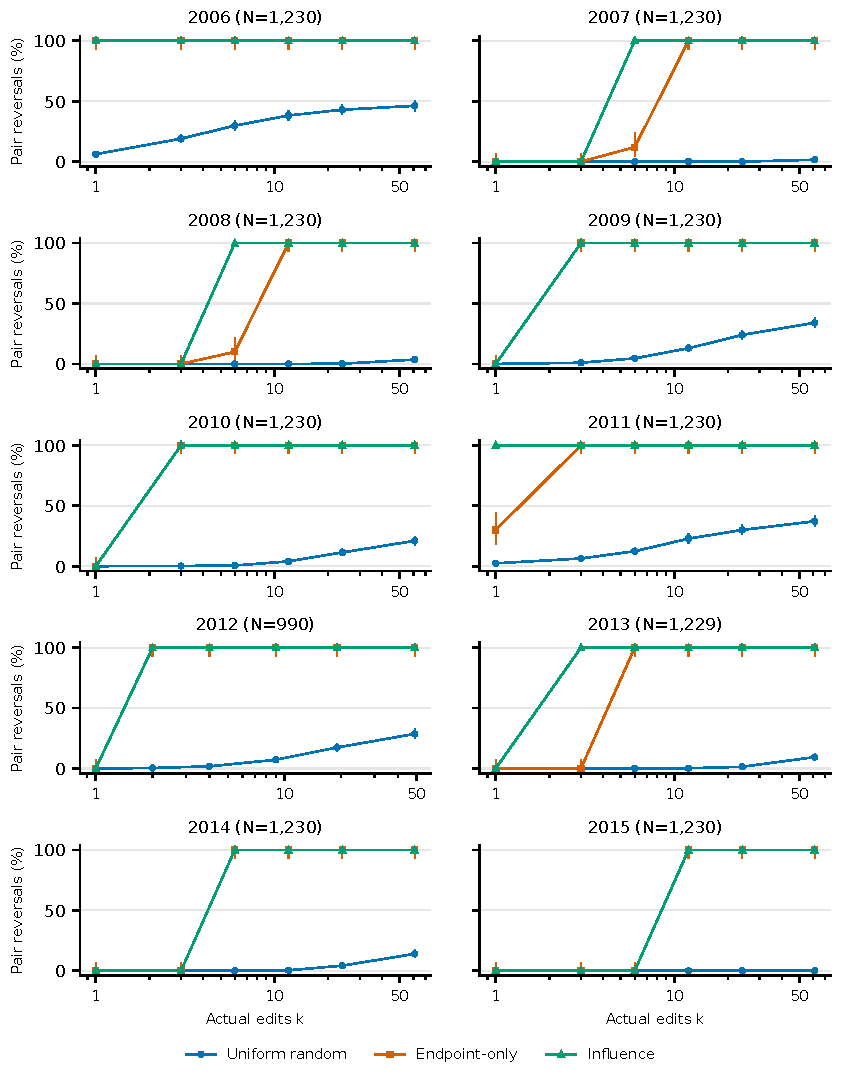
\includegraphics[width=\textwidth]{figures/nba_strategy_curves.pdf}
\caption{\FigNBACaption}
\label{fig:nba}
\end{figure}

\clearpage
